\documentclass{article}
\usepackage[none]{hyphenat}
\usepackage{graphicx}
\usepackage[]{algorithm2e}
\usepackage{program}
\usepackage{eufrak}
\usepackage{amsmath}
\usepackage[a4paper, total={6in, 8in}]{geometry}
\graphicspath{ {images/} }
\begin{document}
	
	\title{Bootstrap Estimation of a Non-Parametric Information Divergence Measure}
	\author { Pradyumna (Prad) Kadambi and Visar Berisha \\
		\small Arizona State University \\
		\small Department of Electrical, Computer and Energy Engineering}
	\date{}
	\maketitle
	
	%----------------------------------------------------------------------------
	\begin{abstract}
		
		This work details the bootstrap estimation of a nonparametric information divergence measure, the $D_p$ divergence measure, applied to the binary classification problem.\ To address the challenge posed by computing accurate divergence estimates given finite size data, the bootstrap approach is used in conjunction with a power law curve to calculate an asymptotic value of the divergence measure estimate. Monte Carlo estimates of $D_p$ are found for increasing values of sample data size, and a power law fit is used to find the asymptotic value of the divergence measure as a function of sample size.\ The fit is also used to generate a confidence interval for the estimate to characterize the quality of the estimator, and the result obtained for the divergence measure is then compared to the result using other resampling methods.\  Using the inherent relation between divergence measures and classification error rate, an analysis of the Bayes error rate of several test data sets is conducted via this power law estimation approach for $D_p$.
	\end{abstract}
	%----------------------------------------------------------------------------
	
	% IDMs are really useful, but they're hard to compute in many cases
	\section{Introduction} 
	$\indent$ Information divergence measures have a wide variety of applications in machine learning, pattern recognition, feature extraction, and big data analysis [8]. The two main classes of information divergence measures are parametric and nonparametric measures. Nonparametric divergence measures, notably including $f$-divergences such as the Kullback-Leibler (KL) divergence,  measure the difference between two distributions $F_0$ and $F_1$.\ Arguably the most well known $f$-divergence, the KL Divergence is a measure of relative entropy and has applications in coding theory, feature selection, and hypothesis testing [20].	Given these wide variety of applications, there is great interest in estimation of $f$-divergences.
	\\ [0.5ex] %write something like this to end the second para
	%Among other applications, it is possible to arrive at bounds for the classification error rate from $f$-divergences [19], so it is of interest to study estimation of $f$-divergences for classification problems.
	
	\indent Normally, when estimating the divergence between two distributions, we have access to independent and identically distributed (i.i.d) training data from each distribution $X_i \in c_0$ and $Y_i \in c_1$ (where $c_0$, $c_1$ correspond to two classes of data). The challenge in estimating the divergence measure between two datasets is that the distributions of the data $F_0$ and $F_1$ are usually unknown. An $f$-divergence, $D_\phi$, is of the form: \begin{equation} D_\phi(F_0, F_1) = \int_{\Omega} \phi\bigg(\frac{dF_0}{dF_1}\bigg)dF_0 \end{equation} given a convex function $\phi(x)$, and feature space $\Omega$ [20].
 	As we lack knowledge of the distribution functions $F_0$ and $F_1$, a direct computation of $D_\phi$ is not possible.
 	\\ [0.5ex]
 	
 	\indent A naive method to calculate the divergence between the data is to first find the densities for $X_i$ and $Y_i$, and then calculate the divergence from the computed density estimates. However, as noted in [5] density estimation adds an undesirable intermediate step before the computation of the divergence measure, introduces additional error, and can be difficult for cases of high dimensionality. 
	\\ [0.5ex]
	
	%PAPER goal paragraph
	\indent	In this paper, we perform a bootstrap estimation of a minimum spanning tree based $f$-divergence derived in [25] using a power law. From data of size $N$, we compute  Monte Carlo iterations at $i$ sample sizes $n\in \{n_1, n_2,... $ $,n_i\}<N$, and apply the unproven, but reasonable assumption that a power law fit can be used to relate the value of the divergence estimator as a function of sample size. We exploit the unique ability to estimate this divergence measure directly from data, and bypass computing the densities. Utilizing this curve we extrapolate as sample size $n\rightarrow\infty$, and find the asymptotic value of the divergence estimate directly from a finite length data set.  As $f$-divergences are be related to the classification error rate, this estimation scheme is applied to binary classification examples to find Bayes error rates for several datasets.
 	%MAybe add 1 sentance about confidence intervals for the estimator
 	\\ [0.5ex]
 	
 	\indent	The work is organized as follows:\ the remainder of Section 1 is devoted to background and previous work. Section 1.1-1.2 discuss $f$-divergences, their connection to the Bayes optimal error rate, and introduce the specific divergence measure used. Section 1.3 discusses the motivation for the bootstrapped power law estimation method, which is formally introduced in Section 2. 
 	%In Section 3 we apply the method to several generated and real-world datasets to show that the power law method can successfully be used to calculate the divergence and classification error rate of several distributions. 
 	In Section 3, examples of the estimation approach are given. In 3.1 we consider generated datasets with known divergence values to demonstrate the accuracy of the estimation algorithm. In 3.2 we perform analysis on the Pima Indians data set and the Banknote data set and compare the calculated Bayes error rate to the classification error rates reported in the literature.
 	%found in the University of California, Irvine machine learning repository [6].
 	%SO, it is difficult to estimate IDMs, so we will get a new method
	%THEN,we will use our method on the Bin Class PRob (BCP), After introducing the BCP, here's why we need to use the method for the BCP
	\subsection*{\ Background and Previous Work}	
	% MST based estimator
	%Work on other divergence measures
	%work on parametric divergence measures
	%the fisher information
	%but we want nonparametric way, therefore
	%work on non parametric divergence measure
	%ASYMPTOTICALLY CONSISTENT
	%kl divergence useful, 
	%thses are all f divergences
	%can use other nonparametric measures such as bhattacharya
	%allow to bound ber
	%dp div eequation
	%		When $f_0(\textbf{x})$ and $f_1(\textbf{x})$ have a common region of support, the classification error rate is greater than zero.
	%----------------------------------------------------------------------------

	\subsection{\ Divergences Measures}
	\subsubsection{\small $f$-divergences}
	%Choice of PHI
	$\indent$ From equation (1), it is clear that $f$-divergences are a function of the distributions of the data from each class.\ In terms of the probability densities $f_0(x)$ and $f_1(x)$, the equation may be rewritten as follows:\begin{equation}
		 D_f(f_0,f_1) = \int_{\Omega} f\bigg(\frac{f_0(\textbf{x})}{f_1(\textbf{x})}\bigg)f_1(\textbf{x})dx
	\end{equation}The resultant divergence is dependent on the choice of $f(x)$.\ For example, the K-L divergence corresponds to $f(x) = -ln(x)$ [6].\  A table of commonly used divergences is given below.
	\begin{table}[ht]
	\caption{Commonly Used $f$-Divergences}
	\centering	
	\begin{tabular}[!h]{ |p{5cm}||p{4cm}|  }
		\hline
		Divergence Measure & $D_f$ \\ 
		\hline\hline
		K-L Divergence 	& $\int f_1(x)ln(\frac{f_0(x)}{f_1(x)})dx$ \\
		
		$L^2$ Divergence & $ \int (f_0(x)-f_1(x))^2dx$ \\
		
		Total Variation Distance & $ \frac{1}{2}\int \vert f_0(x)-f_1(x)\vert dx$ \\
		
		Bhattacharya Distance & $\int\sqrt{f_0(x)f_1(x)}dx$\\ 
		\hline 		
	\end{tabular}	
	\end{table}
	\\ [0.5ex]
	Note that for some cases the divergence may yield values that are not bounded depending on the choice of $f(x)$. 
	%An undefined or unbounded K-L divergence result can be problematic if we then apply the result to a task, and it may be desirable use a bounded divergence measure. 	
%	\\ [0.5ex]
	
	\indent Since in most cases, direct evaluation of the integrals is not possible due to unknown densities, a number of estimation methods have been used to make the problem more tractable. Wang $et$ $al$. [27] derived a nonparametric divergence estimator based on estimating the density ratio $\frac{dF_0}{dF_1}$, and in [28] defined a  $k$-Nearest-Neighbors based divergence estimator that also requires estimates of a density ratio. But, calculation of $\frac{dF_0}{dF_1}$ rather than $f_0(\textbf{x})$ and $f_1(\textbf{x})$ still poses the same drawback: it is undesirable to estimate the divergence by performing the intermediate step of estimating a quantity related to the probability distributions.
	\\ [0.5ex]	
	
	\indent A key advantage of the $f$-divergence we consider is that it can be estimated from the data samples themselves, without intermediate density estimation steps. Towards this end, Hero $et$ $al.$ derive a divergence estimator assuming one of the distributions was known. P{\'o}czos $et$ $al.$ [29] derive estimators for R{\'e}nyi and $L_2$ divergences based on $k$-Nearest Neighbors statistics, and apply the estimate for classifying astronomical data. We consider the $f$-divergence described in [25], which allows for nonparametric estimation directly from sample data via a minimum spanning tree (MST). 
	%It is apparent that when the probability density functions contain no common region of support, the K-L divergence is not bounded. For the total variation distance, $\phi(x) = 0.5 \vert t-1\vert$. Work has
	%Estimation approaches of these measures
	\subsubsection{\small The $D_p$ Divergence Measure}
	$\indent$ The aforementioned divergence for probabilities $p\in (0,1)$, $q=1-p$, and probability densities $f_0$ and $f_1$ is:
	\begin{equation}
			D_p(f_0,f_1)=\frac{1}{4pq}\bigg[ \int \frac{(pf_0(\textbf{x})-qf_1(\textbf{x}))^2}{pf_0(\textbf{x})+qf_1(\textbf{x}))}d\textbf{x}-(p-q)^2 \bigg]
	\end{equation}
	\\[0.5ex]
	
	\indent To classify $D_p$ as a statistical distance, it must satisfy the following properties. Firstly, $0 \leq D_p$, the divergence must be non-negative. Secondly, $D_p=0$ when $f_0(x)=f_1(x)$; the measure between identical distributions must vanish. Third, $D_p(f_0,f_1)=D_p(f_1,f_0)$, it must be symmetric. Fourth,  $D_p(f_0,f_2) \leq D_p(f_0,f_1)+D_p(f_1,f_2)$, the divergence must obey the triangle inequality. $D_p$ is shown in [25] to have the following properties: it is non-negative ($0 \leq D_p \leq 1$ ), satisfies the identity property, and is symmetric. However, the triangle inequality has not been proved for the measure, so therefore, we label $D_p$ as a pseudo-distance.
	\\ [0.5 ex]
	
	\indent The estimator for this divergence relies on finding the Friedman-Rafsky (F-R) test statistic: $\mathcal{C}(\textbf{X}_f,\textbf{X}_g)$ from the $d$-dimensional class data $\textbf{X}_{f_0}$ and $\textbf{X}_{f_1}$. The F-R test statistic is calculated by generating a data set containing both $\textbf{X}_{f_0}$ and $\textbf{X}_{f_1}$, finding the Euclidean MST for the data, and counting the number of edges of the MST that connect a point from $\textbf{X}_{f_0}$ and $\textbf{X}_{f_1}$. The figure below graphically illustrates how the F-R test statistic is calculated: 
	\\ [0.5ex]

	\indent In terms of the F-R test statistic, the estimator for $D_p$ is:
	\begin{equation}
	1 - \mathcal{C}(\textbf{X}_{f_0},\textbf{X}_{f_1})\frac{N_{f_0}+N_{f_1}}{2N_{f_0} N_{f_1}} \rightarrow D_p
	\end{equation}
	as $N_{f0} \rightarrow \infty$ and $N_{f_1} \rightarrow \infty$. Given that $\frac{N_{f_0}}{N_{f_0}+N_{f_1}} \rightarrow p$ and $\frac{N_{f_1}}{N_{f_0}+N_{f_1}} \rightarrow q$. Note that $N_{f0}$ and $N_{f1}$ are the number of samples of data from each class. Using this method, $D_p$ is estimated from the data samples without any density estimation. 
	\\	[0.5 ex]

	\indent In [2] a modified version of this distance is proposed for implementation in binary classification tasks. As binary classification problems are considered in this work, the modified form of the distance, and its estimator are used. Notationally, $\widetilde{D}_p$ is used to refer to the modified divergence, and $D_p$ is used to refer to the distance itself. The same condition that $N_{f0} \rightarrow \infty$ and $N_{f_1} \rightarrow \infty$ is imposed:
	\begin{equation}
		\widetilde{D}_p(f_0,f_1)=\int \frac{(p{f_0}(\textbf{x})-q{f_1}(\textbf{x}))^2}{p{f_0}(\textbf{x})+q{f_1}(\textbf{x}))}d\textbf{x}
	\end{equation}
	\begin{equation}
	1 - 2 \frac{\mathcal{C}(\textbf{X}_{f_0},\textbf{X}_{f_1})}{N_{f_0} + N_{f_1}} \rightarrow \widetilde{D}_p(f_0,f_1)
	\end{equation}
%	\\ [0.5ex]
	Note that this quantity is not a distance, as in the case of $f_0(\textbf{x})=f_1(\textbf{x})$, it does not satisfy the identity property. However, (5) is estimated rather than (3) as it leads to Bayes error rate bounds that are simpler. Additionally, it is easily seen that when $p=q=0.5$, the identity condition $is$ met for $\widetilde{D}_p$, and for that case $\widetilde{D}_p=D_p$. For all the cases we consider, $p=q=0.5$. Therefore, $\widetilde{D}_p$ and $D_p$ are equivalent in the context of this work.
	
	\subsection{\ Bayes Error Rate and Divergence Measures}
	$\indent$ A common problem in machine learning is binary classification, in which data $\textbf{X}_i\in \mathbf{R^{n \times d}}$ are assigned a class label $c_i \in \{0,1\}$.
	Given $c_0$ and $c_1$ correspond to data with respective probability distributions $f_0(\textbf{x})$ and $f_1(\textbf{x})$, prior probabilities $p \in (0,1)$ and $q=1-p$, the Bayes optimal classifier assigns class labels to $x_i$ such that the posterior probability is maximized [4].\ The error rate of this optimal classifier, the Bayes error rate (BER), provides an absolute lower bound on the classification error rate.\ Accurate estimation of the BER makes it possible to quantify the performance of a classifier with respect to this optimal lower bound, or apply improved BER bounds to feature selection algorithms [1]. 
	\\ [0.5ex]
	
	\indent Given the two conditional density functions, $f_0(\textbf{x})$ and $f_1(\textbf{x})$, it is possible to write the Bayes error rate in terms of the prior probabilities $p$ and $q$:
	%insert bayes error rate equation here
	\begin{equation} E_{Bayes}=\int_{r_1} pf_0(\textbf{x}) \,d\textbf{x} + \int_{r_0} qf_1(\textbf{x}) \,d\textbf{x} \end{equation}
	%ADD PROPER LIMITS TO INTEGRAL
	\indent Here, $r_1$ and $r_0$ refer to the regions where the respective posterior probabilities are larger.\ Direct evaluation of this integral can be quite involved and impractical, and poses similar problems to that of estimation of $f$-divergences: it is challenging to create an exact model for the distributions $f_0(\textbf{x})$ and $f_1(\textbf{x})$.\ As an alternative to direct evaluation of the integral, it is possible to derive bounds for the Bayes error rate in terms of divergences measures [5]. 
	\\ [0.5ex]	
	
	\indent The Bayes error rate can be related to the total variation distance (shown in Table 1), which itself can given in terms of the K-L divergence [30], [31]. The Pinkser inequality [32] and related bounds are one such method to arrive at the total variation distance from the K-L divergence. However, as noted previously, in certain cases the K-L divergence may not be bounded, and can result in a value that tends to $\infty$. Vajda [33] modified the relation between the K-L divergence and the total variation distance to account for this problem. 
	\\	[0.5 ex]
	$\indent$Bounds for the classification error rate have been given in terms of the Bhattacharya distance in [33]. In [2] the Bayes error rate is given in terms $\widetilde{D}_p$:\begin{equation}
	\frac{1}{2}-\frac{1}{2}\sqrt{\widetilde{D}_p(f_0,f_1)}\leq E_{Bayes} \leq \frac{1}{2}-\frac{1}{2}\widetilde{D}_p(f_0,f_1)
	\end{equation}
	As expected, when there is no overlap between the two distributions, $\widetilde{D}_p=1$, and the BER is lower bounded by zero. In other words, if the two classes are highly separated, it should be possible to design a classifier that has a very low probability of error. On the other hand, if there is full overlap between the two distributions, $\widetilde{D}_p=0$, and the BER is $0.5$. The optimal error rate is equivalent to the error in randomly assigning class.  
	\subsection{\ Bootstrap Estimation Based on Power Law}
	$\indent$ As we have just shown, the method for empirically calculating a specific ${D}_p$ value for a data set of length $N$, and obtaining an estimate for the BER is quite straight forward, but it leaves much to be desired. Specifically, it is necessary to characterize the quality of the ${D}_p$ estimate. A direct calculation of the divergence measure using all $N$ data points yields only a single value, and does not provide any insight into the error or spread of  the statistic. Indeed, in many cases knowledge of the spread of the estimate is as important as the estimate itself.
	\\[0.5ex]
	
	\indent Bootstrap resampling, first introduced by Efron in [10], is a powerful tool to find the spread of an estimator. From a data set $\textbf{X}_i$ of size $N$, the bootstrap method functions by repeatedly and randomly sampling, with replacement, $b$ subsets of size $n<N$ from the original data set. Then estimates are computed for all $b$ generated subsets. This Monte Carlo approach gives a powerful way to analyze some measure of estimator quality from $b$ estimates. However, the bootstrap with replacement fails when applied to the F-R test statistic based estimator. Because the F-R test statistic requires the generation of unique distances between data points when computing the minimum spanning tree, it is not desirable to sample with replacement [2]. 
	% we denote $S(\textbf{X}_i)$.
	%bootstrapping is great, it gives us this spread knowledge, but
	% we also want to apply this estimation method into 
	\\ [0.5ex]
	
	%Explain why we want a CI for D_p
	\indent To satisfy this requirement, we consider another bootstrap resampling technique, the $m$ out of $N$ bootstrap, that generates $b$ randomly sampled subsets of size $m<N$, $without$ $replacement$, in order to obtain a sense of the distribution of the estimator. Particularly, we consider the confidence interval of ${D}_p$. Now, we have an estimate of ${D}_p$ along with a confidence interval. But, this estimate is for finite data size, and the estimator for ${D}_p$, equation (6), specifies an asymptotic condition of $N_{f0} \rightarrow \infty$ and $N_{f_1} \rightarrow \infty$. Obtaining this estimate of ${D}_p$ for $N \rightarrow \infty$ is desirable in order to minimize the bias. 
	\\ [0.5ex]
	
	\indent Hawes and Priebe [1] applied a $k$-Nearest Neighbors rule to find the upper and lower bound on the asymptotic Bayes error rate as a function of sample size. They perform bootstrap estimates of the BER (which they denote as $\bar{L}_n(k)$) at sample sizes $n_1 \textless n_2 \textless ... \textless n_i \textless N$. Then they apply a parametric power law curve to calculate the bootstrapped Bayes error rate estimates as a function of sample size, $n$:
		\begin{equation}
		\bar{L}_n(k)=an^b+c
		\end{equation}
	with power law fit constants $a$, $b$, $c$, and sample size $n$. Given that this model is valid, $b<0,$ and as $n \rightarrow \infty$, $\bar{L}_n(k)\rightarrow c$ with $c=\bar{L}_\infty(k)$. In [34] it is shown that $\vert \bar{L}_n(1)-\bar{L}_\infty (1) \vert \leq an^{-2}$; the absolute error of the BER estimate for a 1-dimensional data, with $k=1$ rule, converges in the form given by equation (9). 
	\\[0.5ex]
	
	\indent This result was generalized in [35] for $d$-dimensional data. In [36] was generalized to any choice of $k$, and produced the following expression for the BER:
	\begin{equation}
	\bar{L}_n(k)~\bar{L}_\infty (k) + \sum_{j=2}^{\infty} c_j n^{-j/d}
	\end{equation}
	As $n$ increases, the term that dominates happens to be $cn^{-2/d}$. This is in agreement with the earlier described result for the $d=1$ case. (Please note that for the remainder of this paper, the Bayes error rate will be referred to as $E_{Bayes}$, not $\bar{L}_n(k)$).

	\section{Methods}
	
	\indent While Hawes and Priebe focus on obtaining asymptotic bounds of the BER, this works focuses on finding the asymptotic value for the ${D}_p$ estimator. As shown in equation (8) of Section 1.2, it is possible to simply and directly relate the Bayes error rate to ${D}_p$. Therefore, the motivation behind the power law method for bounding the BER can also motivate an approach to find ${D}_p$. Though it has not been proven, it is a sensible assumption that the divergence estimates follow a similar power law for increasing sample size, and that an asymptotic estimate,  $\bar{D}_p^*$,  may be generated using this formulation. The following power law is used:
	\begin{equation}
		\bar{D}_p(f_0,f_1)=an^b+c
	\end{equation}

	\indent Notice that under the sound assumption of $b<0$, $\bar{D}_p^* \rightarrow c$ as $n \rightarrow \infty$. So, we have good reason to believe that from a size $N$ finite length data set, it is possible to obtain asymptotic estimates for the divergence. To find a measure of spread for the divergence estimator, the 95\% confidence interval calculated from the curve fitting process. Reviewing notation, $D_p$ refers to the distance in equation (3), $\widetilde{D}_p$ is the modified version of the distance suited to binary classification given in equation (5), and is equivalent to $D_p$ for our cases. $\bar{D}_p$ is the power law curve describing the estimator of ${D}_p$ as a function of sample size from the equation above. The asymptotic value of the divergence is denoted as $\bar{D}_p^*$.
	
	%While the $D_p$ value provides an insight into the separation of the data, as stated prevopu   
%	Given a data set of size $N$ and dimensionality $D$, we have established how to calculate the $D_p$ value. How
	%limitation of sample size
	% why we want the aasymptotic boostrap
	% we can get the bias for the current value of D_p
	%Information divergence measures have a wide variety of applications in machine learning, pattern recognition, feature extraction, and big data analysis [8].  The two main classes of %information divergence measures are parametric and nonparametric measures.\ Parametric divergence measures are functions of an unknown parameter $\theta$, and describe the information %contained in the data about $\theta$[18].\ Nonparametric divergence measures measure the difference between two distribution functions $f_0$ and $f_1$. Due to their wide range of %sapplications, there has been particular interest in estimation of these information theoretic quantities, particularly in the machine learning literature [10-14].
	%	CHANGE THIS PARAGRAPH
	%	\indent Equally important to estimating the divergence measures, is obtaining a metric of estimator quality, such as variance or 95\% confidence interval. Before the estimator is applied in data analysis, knowledge of its approximate sampling distribution is critical in quantifying its usefulness. We analyze a nonparametric, asymptotically consistent divergence measure and apply it to the binary classification task.
	%	CHANGE THIS PARAGRAPH
	% Need some paragraph here
	%\subsection*{\small The Binary Classification Problem}
	%\indent We arrive at an estimate of the Bayes error rate by using expressions that give bounds on the classification error in terms of information divergence measures. However, common methods of estimating the Bayes error rate via divergence measure still require information about the conditional distributions corresponding to both class labels.\ Therefore the nonparametric divergence measure given in [3] will be used in conjunction with the Bayes error estimates derived for this divergence measure in [2] to conduct the analysis.     
	
	\subsection{Algorithm for $\bar{D}_p^*$ Calculation}
	\begin{algorithm}[H]
		\caption{Algorithm for finding asymptotic divergence value $\bar{D}_p^*$}
		\SetKwInOut{Input}{Input}
		\SetKwInOut{Output}{Output}
		\KwIn{Data $\textbf{X}_0,\textbf{X}_1 \in$ $\mathbf{R^{n\times d}}$  of length $N$, dimensionality $\textbf{d}$ \newline $m$: number of Monte Carlo iterations \newline $i$: number of bootstrap subsample sizes $\textbf{n}_i \in \{n_1, n_2, ... ,n_i \textless N$\} \newline $\textbf{X}_S=\textbf{X}_0 \bigcup \textbf{X}_1$}		
		
		\KwResult{Asymptotic estimate of ${D}_p$ : $\bar{D}_p^*$ \newline Power law curve: $ \mathcal{P}(\bar{\textbf{D}}_{p_i},\textbf{n}_i) = \bar{D}_p(f_0,f_1)=an^b+c$}
		
		$\newline$	
		\textbf{Define: } 
		$\bar{\textbf{D}}_{p_i}=\{\bar{D}_{p_1},\bar{D}_{p_2},...,\bar{D}_{p_i} \}$, bootstrapped estimate for each sample size $n_i$
		
		$\newline$
		\For{$i\in$ $n_1, n_2, ..., n_i$}{
		$\newline$
			Define empty array ${\textbf{D}}_{p}=\{{D}_{p_1},{D}_{p_2},...,{D}_{p_m} \}$, containing the $m$ Monte Carlo estimates
			
			$\newline$			
			\For{$k \in 1 ... m$}{
  				 Randomly sample a length $n_i$ subset: $\textbf{S}=\{x_1, ..., x_{n_i}\}$ from $\textbf{X}_S$, without replacement 
				$\newline$ // Ensure $N_{S,0}=N_{S,1}$, number of data samples from each class must be equal
				$\newline$ $\newline$
				// Compute $k^{th}$ Monte Carlo estimate
				$\newline$${D}_{p_k}=1 - 2 \frac{\mathcal{C}(\textbf{S}_{0}, \textbf{S}_{1})}{N_{S,0} + N_{S,1}} $ $\indent$  $\indent$  $\indent$
				}
			// Bootstrapped estimate $\bar{D}_{p_i}$ is the average of the ${D}_{p_k}$
			$\newline$ $\bar{D}_{p_i} = \frac{1}{m}\sum_{k=1}^{m}{D}_{p_k}$  $\indent$ $\indent$ $\indent$
	
	}
	$\newline$
	// Apply the power law 
	
	$ \{a,b,c\} = \mathcal{P}(\bar{\textbf{D}}_{p_i},\textbf{n}_i)$ 

	$\bar{D}_p^*=c$
	\end{algorithm}
	$\\[0.5ex]$
	
	$\indent$	The algorithm for finding the $\bar{D}_p^*$ value for a two class data set, follows from the overview of bootstrap sampling in 1.3. Then $m$, the number of Monte Carlo iterations, must be defined. Choose, $i$ and $\textbf{n}_i$, the number of bootstrap subsamples and the bootstrap subsample sizes. Begin with the outer loop, and iterate through the number bootstrap subsample sizes, $i$. Create a randomly sampled subset $\textbf{S}$ of length $n_i$ from the data $\textbf{X}_S$ containing an equal number of elements from each class, and compute the divergence estimate for the subset $\textbf{S}$. Repeat the subset creation and divergence estimation $m$ times (this is the inner loop). Upon returning to the outer loop, find the mean of the $m$ $D_{p_k}$ values. Once the mean value of $m$ estimates for all $i$ bootstrap subsample sizes has been found, apply the power law fit, $\mathcal{P}$, to the mean values and subsample sizes. The asymptotic value of the divergence estimator $\bar{D}_p^*$ is equal to $c$.
	
	$\indent$ We note several restrictions on input parameters. Define maximum value of subsample size as $n_{max}$. This value must be less than $N$. Also, $\binom{N}{n_{max}}>m$. This is a requirement for sensible Monte Carlo iterations: there must be at least $m$ unique subsets of size $n_{max}$. From the lower extreme of subsample size, $n_1$ must be greater than the number of dimensions of the data set.

	
	\section{Results}
	\subsection{\small Uniform Dataset}
	$\indent$ To test the operation of the estimation algorithm, a data set with a known divergence is constructed in order to ensure that the computed value of $\bar{D}_p^*$ matches with the known divergence. For this purpose, the uniform distribution shown in Table 2 is defined. The data set contains 8 dimensions, all of which have variance $\sigma^2=\frac{1}{12}$, and are uniformly distributed along $[-0.5,0.5]$, with the exception of one dimension from $c_1$. That dimension has an offset mean of $\mu_1=\frac{1}{2}$ rather than  $\mu_1=0$. It is easy to see that a direct application of equation (3) or (5) results in a divergence value of $D_p=0.5$. Refer to the Appendix for this computation.
	\begin{table}[ht]
		\caption{Uniform Dataset for Bootstrap Analysis of $D_p$}
		\centering % used for centering table
		\begin{tabular}{c c c c c c c c c c} % centered columns (4 columns)
			%inserts double horizontal lines
			$c_0$ &  &  &  \\ [0.5ex] % inserts table
			%heading
			\hline % inserts single horizontal line
			$\mu_0$ & 0 & 0 & 0 & 0 & 0 & 0 & 0 & 0\\[0.5ex] % inserting body of the table
			$\sigma_0^2$ & \( \frac{1}{12} \) & \( \frac{1}{12} \) & \( \frac{1}{12} \) & \( \frac{1}{12} \) & \( \frac{1}{12} \) & \( \frac{1}{12} \) & \( \frac{1}{12} \) & \( \frac{1}{12} \) &  \\[2ex]
			
			$c_1$ & \\ [0.5ex]
			
			\hline
			$\mu_1$ & \( \frac{1}{2} \) & 0 & 0 & 0 & 0 & 0 & 0 & 0\\[0.5ex] % inserting body of the table
			$\sigma_1^2$ & \( \frac{1}{12} \) & \( \frac{1}{12} \) & \( \frac{1}{12} \) & \( \frac{1}{12} \) & \( \frac{1}{12} \) & \( \frac{1}{12} \) & \( \frac{1}{12} \) & \( \frac{1}{12} \) &  \\ [1ex] % [1ex] adds vertical space
			\hline %inserts single line
		\end{tabular}
		\label{table:nonlin} % is used to refer this table in the text
	\end{table}
	\begin{figure}[h!]
			\caption{Asymptotic Convergence of $D_p$ for 8-Dimensional Uniform Data Set, m = 200 trials}
			\centering
			%	\begin{center}
			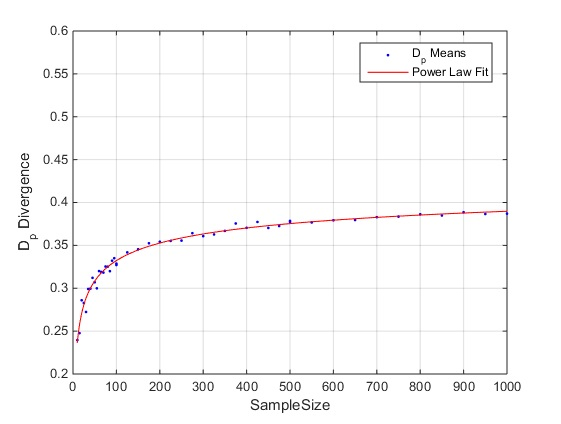
\includegraphics[scale=0.6]{dp_n200_uniform}
			%	\end{center}
	\end{figure}	
	$\newline$
	$\indent$ To find $\bar{D}_p^*$, a 10000 point dataset containing an equal number of instances from both classes $c_0$ and $c_1$ was created. With respect to Algorithm 1, the parameters of the simulation were: $N=10000$, $m=200$ Monte Carlo iterations, $i=50$ bootstrap subsample sizes, and $n_{50}=1000$ as the maximum bootstrap sample size. The results of the simulation are shown in Figure 1. The plot shows computed estimates of $D_p$ as a function of sample size and displays the resulting power law fit. Each blue point on the figure is a $D_p$ mean - the mean of 200 Monte Carlo trials at each bootstrap sample size $n_i$.
	\\[0.5ex]

	$\indent$ The power law found for $D_p$ for this uniform dataset is:
	
	\begin{equation}
	\bar{D}_p=-0.39n^{-0.22}+0.4775
	\end{equation}
	The asymptotic estimate $\bar{D}_p^*=0.4775$ agrees with the analytically calculated value for the dataset, ${D}_p=0.5$. To understand the true capability of the power law based, asymptotic estimation method consider Table 3.
	
	\begin{table}[!h]		
		\caption{Estimated $D_p$ for Uniform Data Set for $n_{max}=1000$ [4]}
		\begin{center}
			%	\begin{tabular}{||c c c c||} 
			%		\hline
			\begin{tabular}[!h]{ |p{5cm}||p{4cm}|  }
				\hline
				Value & Result\\ [0.5ex] 
				\hline\hline
				$D_p$ (no Bootstrap) & $0.3370$ \\
				$\bar{D}_p$ & 0.3870 (0.3646, 0.4064) 	\\
				$\bar{D}_p^*$ & $\textbf{0.4775}$  (0.4378, 0.5173)\\ 
				$D_p$ (true value) & 0.5 \\
				\hline 		
			\end{tabular}
		\end{center}
	\end{table}
	When a direct computation of the divergence measure is performed for 1000 data points an estimate of $D_p=0.337$ is obtained. This is problematic for two reasons. As explained earlier, there is no information about the distribution of the estimate. Additionally, the calculated value $D_p=0.337$, is far from the true value of $D_p=0.5$. 
	
	\subsubsection*{Proper Selection of $\textbf{n}_i$}
	$\indent$ While selecting the set of subsample sizes $\textbf{n}_i \in \{n_1, n_2,... ,n_i<N\}$, it is vital that a significant portion of the $i$ subsample sizes are concentrated within the rapidly rising portion of the power law curve. In Figure 1, notice that for a sample size of up to $n=200$, the estimates of divergence change rapidly for increasing sample size. But, for $n>200$, the convergence of the estimates slows - the divergence estimates change slowly for increasing sample size. In this case the $n_i$ are chosen so that $n_1$ to $n_{20}$ are spaced evenly on the interval $[8,100]$ ($n_1$ should not be smaller than the number of dimensions). Then, $n_{21}$ to $n_{40}$ are evenly spaced for $[100,500]$. Finally, $n_{41}$ to $n_{50}$ are evenly spaced between $[500,1000]$. 
	\\[0.5ex]	
	
	$\indent$ Although the exact choice of $\textbf{n}_i$ may differ between each use case, a useful heuristic to ensure a good power law fit is described. Take the maximum bootstrap subsample size to be $n_{max}<N$. In this case, $n_{max}=1000$. Choose approximately $\frac{1}{3}$ of the $n_i$ subsamples on the interval $(0,0.1n_{max})$, choose $\frac{1}{3}$ of the subsamples between $(0.1n_{max}, 0.5n_{max})$, and choose the final $\frac{1}{3}$ in the interval $(0.5n_{max}, n_{max})$. If there are fewer number of subsamples $n_i$ that are small relative to $n_{max}$, or if $n_i$ are evenly spaced along $(0,n_{max})$, the goodness of fit for the power law is likely to be compromised. If $n_i$ must be evenly spaced, we may increase the number of subsamples, $i$, and decrease the space between each subsample size to try and preserve a good curve fit.   
	\\[0.5ex]
	
	\begin{figure}[h!]
		\caption{Distribution of $D_p$ Values for 8-Dimensional Uniform Data Set, m = 200 trials}
		\centering
		%	\begin{center}
		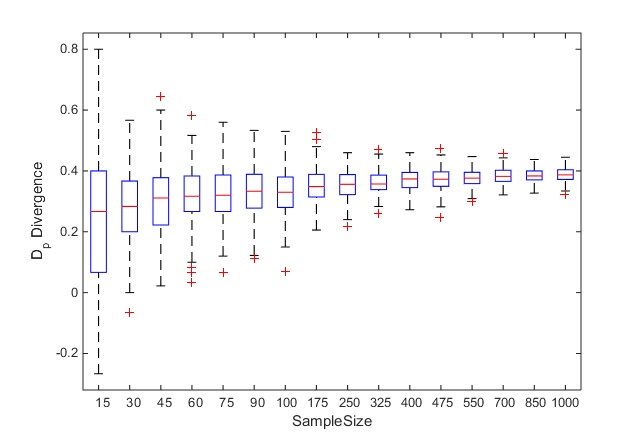
\includegraphics[scale=0.6]{dp_n200_uniform_bars}
		%	\end{center}
	\end{figure}
	
	$\indent$ An additional benefit of increasing the subsample size, is that the spread of estimator decreases. The same data used to create Figure 1 are shown in Figure 2 to emphasize the decrease in estimator's spread. Recognize that the x-axis is not linearly scaled, and that the y-axis does not have the same scale as Figure 1. For every $D_p$ point plotted in Figure 1 (every blue point), $m=200$ Monte Carlo estimates have been averaged.	In Figure 2, box plots of the Monte Carlo iterations are shown for select values of subsample size. Although every single average $D_p$ value plotted in Figure 1 has a corresponding box plot, only a select number of box plots are shown due to limited space, and to avoid cluttering the Figure. Here, the estimator's bias for small sample sizes is clearly visible in the $n=15$ case, as negative values are produced. But, as sample size increases, a dramatic reduction in the interquartile range of the $n$.
	\newpage	
	
	
	
\newpage
	\subsection{\small Gaussian Dataset}
	
	
	\begin{table}[!h]
		\caption{Gaussian Dataset for Bootstrap Analysis of $D_p$}
		\centering % used for centering table
		\begin{tabular}{c c c c c c c c c c} % centered columns (4 columns)
			%inserts double horizontal lines
			$D_0$ &  &  &  \\ [0.5ex] % inserts table
			%heading
			\hline % inserts single horizontal line
			$\mu_0$ & 0 & 0 & 0 & 0 & 0 & 0 & 0 & 0\\[0.5ex] % inserting body of the table
			$\sigma_0$ & 1 & 1 & 1 & 1 & 1 & 1 & 1 & 1\\[0.5ex]
			
			$D_1$ & \\ [0.5ex]
			
			\hline
			$\mu_1$ & 0 & 0 & 0 & 0 & 0 & 0 & 0 & 0\\[0.5ex] % inserting body of the table
			$\sigma_1$ & 2.56 & 1 & 1 & 1 & 1 & 1 & 1 & 1\\[0.5ex]
			\hline %inserts single line
		\end{tabular}
		\label{table:nonlin} % is used to refer this table in the text
	\end{table}
	
	\begin{figure}[h!]
		\caption{Asymptotic Convergence of $D_p$ for Gaussian Data Set, N = 50 trials}
		\centering
		%	\begin{center}
		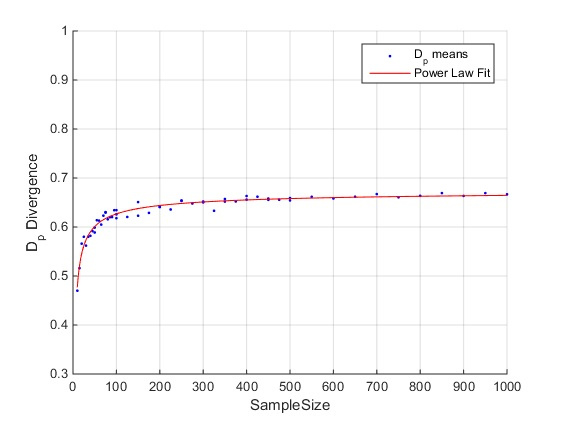
\includegraphics[scale=0.6]{dp_n50_gaussian}
		%	\end{center}
	\end{figure}	
	

	
	\newpage


	\subsection{\small Banknote Dataset}
	\indent The empirical example we consider is the Banknote Authentication Data Set taken from the University of California, Irvine Machine Learning Repository [7]. The 4-dimensional dataset contains data extracted from images of banknotes. The dataset consists of a relatively small number of dimensions, and highly separated data, so the convergence is rapid, even for relatively small sample size. We note that for a sensitive task such as authenticating banknotes, it should not be surprising to see an asymptotic value for $D_p$ that is close to 1, indicating that the classes are well separated.  
	\begin{figure}[h!]
			\caption{Convergence of $D_p$ for Banknote Authentication Data Set, N = 50 trials}
			\centering
			%	\begin{center}
			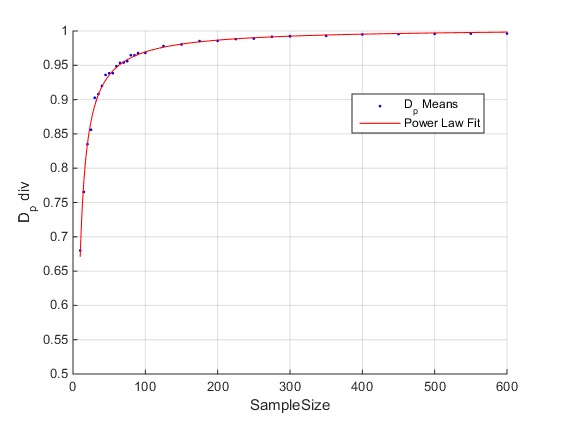
\includegraphics[scale=0.6]{dp_n50_banknote}
			%	\end{center}
	\end{figure}

	\subsection{\small Pima Indians Dataset}
	
	\begin{figure}[!h]
		\caption{Asymptotic Convergence for Pima Indian Data Set, N = 50 trials}
		\centering
		%	\begin{center}
		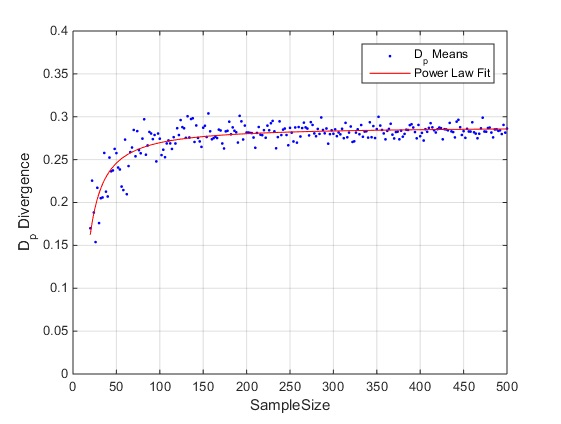
\includegraphics[scale=0.6]{dp_n50_pima}
		%	\end{center}
	\end{figure}
	
	\begin{figure}[!h]
		\caption{Asymptotic Convergence for Pima Indian Data Set, N = 200 trials}
		\centering
		%	\begin{center}
		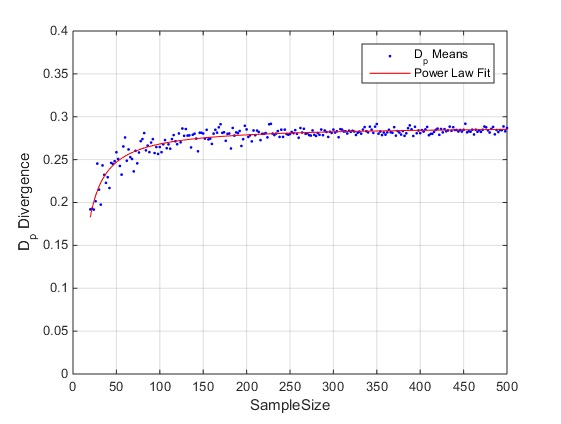
\includegraphics[scale=0.6]{dp_n200_pima}
		%	\end{center}
	\end{figure}	
	
	\begin{figure}[!h]
		\caption{Asymptotic Convergence for Pima Indian Data Set, N = 5000 trials}
		\centering
		%	\begin{center}
		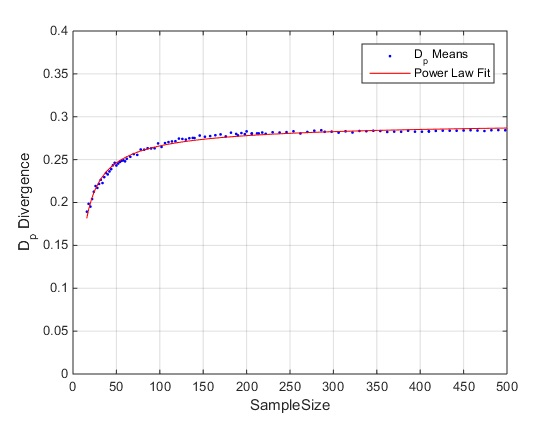
\includegraphics[scale=0.6]{dp_n5000_pima}
		%	\end{center}
	\end{figure}	
	
	%		\begin{figure}[!h]
	%			\caption{Asymptotic Convergence for Pima Indian Data Set, N = 5000 trials}
	%			\centering
	%			%	\begin{center}
	%			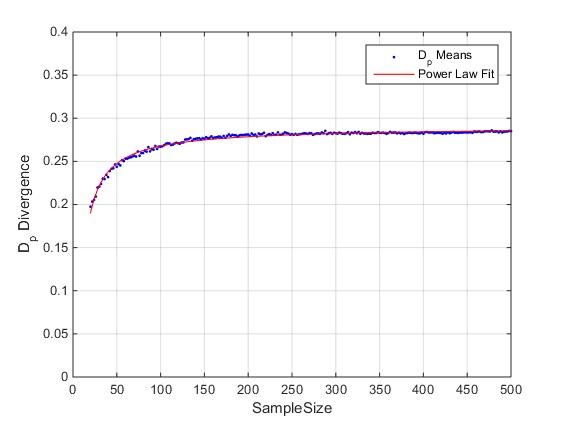
\includegraphics[scale=0.75]{dp_n5000}
	%			%	\end{center}
	%		\end{figure}	
	
	\newpage
	\begin{table}[!h]		
		\caption{Bayes Error Rates in Literature for Pima Indians Data Set [4]}
		\begin{center}
			%	\begin{tabular}{||c c c c||} 
			%		\hline
			\begin{tabular}[!h]{ |p{5cm}||p{4cm}|  }
				
				\hline
				Algorithm & Bayes Error Rate (\%) \\ [0.5ex] 
				\hline\hline
				
				Discrim & 22.50	\\
				Quadisc &  26.20	\\
				Logdisc &  22.30	\\
				SMART  & 23.20	\\
				ALLOC80 &  30.10	\\
				K-NN  & 32.40	\\
				CASTLE &  25.80	\\
				CART  & 25.50	\\
				IndCART &  27.10	\\
				NewID &  28.90	\\
				AC2 &  27.60	\\
				Baytree  & 27.10	\\
				NaiveBay &  26.20	\\
				CN2  & 28.90	\\
				C4.5  & 27.00	\\
				Itrule &  24.50	\\
				Cal5  & 25.00	\\
				Kohonen &  27.30	\\
				DIPOL92 &  22.40	\\
				Backprob  & 24.80	\\
				RBF  & 24.30	\\
				LVQ  & 27.20 	\\ 
				
		%		\textbf{$D_p$}  \\
		%		\textbf{$D_p$ Asymptotic Power Law} & \textbf{22.83} \\ 
				\hline 		
			\end{tabular}
		\end{center}
	\end{table}
	
	
		
	\begin{table}[!h]		
		\caption{Bootstrap Estimated Bayes Error Rates for Pima Indians Data Set [4]}
		\begin{center}
			%	\begin{tabular}{||c c c c||} 
			%		\hline
			\begin{tabular}[!h]{ |p{5cm}||p{4cm}|  }
				\hline
				Algorithm & Bayes Error Rate (\%) \\ [0.5ex] 
				\hline\hline
						$D_p$ (no Bootstrap) & $29.32 \pm 6.22$ * \\
						Efron Bootstrap  & $14.87 \pm 2.465$ ** 	\\
						$m < n$ Bootstrap, $m=200$ & $23.13 \pm 4.13$ 	\\
				\textbf{$D_p$ Asymptotic Power Law} & $\textbf{22.78} \pm \textbf{0.11}$\\ 
				\hline 		
			\end{tabular}
		\end{center}
	\end{table}
	
	\newpage
	\begin{table}[!h]		
		\caption{$D_p$ and Bayes Error Rate for the Pima Indian Data Set for Increasing Sample Size, and Increasing Monte Carlo Iterations}
		\begin{center}
			%	\begin{tabular}{||c c c c||} 
			%		\hline
			\begin{tabular}[!h]{ |p{1cm}||p{1.5cm}|p{4cm}|p{3.5cm}| |p{3.5cm}| }
				
				\hline
				Sample Size & Monte Carlo Iterations & $D_p$ Asymptotic Value $\newline$(95\% Confidence Interval)& Bayes Error Rate (\%),$\newline$ ($\pm$ 95\% CI) $\newline$ Lower Bound &   Bayes Error Rate (\%),$\newline$ ($\pm$ 95\% CI) $\newline$ Upper Bound \\[0.5ex] 
				\hline\hline
				100	& 50	& 0.2725   (0.245, 0.3)	& $23.90  \pm 1.32$		 &  $36.38  \pm 1.38$\\
				
				\hline
				
				100	& 200	& 0.2958  (0.265, 0.3267)	& $22.81  \pm 1.42$   &$35.21  \pm 1.54$\\
				\hline
				
				100	& 5000	& 0.3107  (0.2959, 0.3254)	& $22.13  \pm 0.67$   &$34.47  \pm 0.75$\\
				
				\hline
				200	& 50	& 0.2946  (0.2732, 0.3161)	& $22.86  \pm 0.99$   &$35.27  \pm 1.07$\\
				
				\hline 
				200	& 200	& 0.3029  (0.288, 0.3178)	& $22.48  \pm 0.68$   &$34.86  \pm 0.74$\\
				
				\hline
				200	& 5000  & 0.3162  (0.3114, 0.3209)	& $21.88  \pm 0.21$   &$34.19  \pm 0.24$\\
				
				\hline
				300	& 50	& 0.3118  (0.2827, 0.3409)  & $22.08  \pm 1.31$   &$34.41  \pm 1.46$\\
				\hline
				300	& 200	& 0.3073  (0.2926, 0.3219)	& $22.28  \pm 0.66$   &$34.63  \pm 0.74$\\
				\hline
				300	& 5000	& 0.3041  (0.3006, 0.3075)	& $22.43  \pm 0.16$   & $34.79  \pm 0.18$\\ 
				\hline 	
				500	& 50	& 0.2886  (0.2855, 0.2917)  & $23.14  \pm 0.14$   &$35.57  \pm 0.15$\\
				\hline
				500	& 200	& 0.2895  (0.2871, 0.2918)	& $23.10  \pm 0.11$   &$35.53  \pm 0.12$\\
				\hline
				500	& 5000	& 0.2963  (0.2939, 0.2987)	& $22.78  \pm 0.11$   &$35.19  \pm 0.12$\\ 
				\hline
					
			\end{tabular}
		\end{center}
	\end{table}			
	%	\newpage
	%		\section{Conclusion}
	
%	\Needspace{5\baselineskip}
	\newpage
	\section*{References}
	\noindent [1] Hawes, Chad M., and Carey E. Priebe. "A Bootstrap Interval Estimator for Bayes' Classification 
	\indent Error." 2012 IEEE Statistical Signal Processing Workshop, 2012
	\\ [0.5ex]
	
	\noindent[2] V. Berisha, A. Wisler, A.O. Hero, and A. Spanias, "Empirically Estimable Classification Bounds 
	\indent Based on a Nonparametric Divergence Measure" IEEE Transactions on Signal Processing, vol. 
	\indent 64, no. 3, pp.580-591, Feb. 2016.
	\\ [0.5ex]
	
	\noindent[3] A. O. Hero, B. Ma, O. Michel, and J. Gorman, “Alpha-divergence for classification, indexing 
	\indent and retrieval,” Communication and Signal Processing Laboratory, Technical Report CSPL-328, 
	\indent U. Mich, 2001
	\\ [0.5ex]
	
	\noindent [4] K. Tumer, K. (1996) "Estimating the Bayes error rate through classifier combining" in Proceedings 
	\indent of the 13th International Conference on Pattern Recognition, Volume 2, 695–699
	\\ [0.5ex]
	
	\noindent[5] Tumer, Kagan, and Joydeep Ghosh. "Bayes Error Rate Estimation Using Classifier Ensembles." 
	\indent International Journal of Smart Engineering System Design 5.2 (2003): \indent 95-109.
	\\ [0.5ex]
	
	\noindent[6] Lichman, M. (2013). UCI Machine Learning Repository [http://archive.ics.uci.edu/ml]. Irvine, 
	\indent CA: University of California, School of Information and Computer Science.
	\\ [0.5ex]
	
	\noindent [7] V. Lohweg, “Banknote Authentication Data Set,” 2012. [Online]. Available: https://archive.ics.uci.edu/ml/datasets/banknote+authentication.
	\\ [0.5ex]
	
	\noindent [8] K. Pranesh, and L. Hunter. "On an Information Divergence Measure and Information Inequalities." (n.d.): n. pag. University of Northern British Columbia. 
	\\ [0.5ex]
	
	\noindent [9] Tukey, J.W. 1958. Bias and confidence in not-quite large samples. Annals of Mathematical 
	\indent Statistics 29: 614
	\\ [0.5ex]
	
	\noindent [10] Efron, B. "Bootstrap Methods: Another Look at the Jackknife." Annals of Statistics 7.1 (1979)
	\\ [0.5ex]
	
	\noindent [11] https://www.princeton.edu/~verdu/reprints/WanKulVerSep2005.pdf **Create Citation
	\\ [0.5ex]
	
	\noindent [12] http://www.princeton.edu/~verdu/reprints/WanKulVer.May2009.pdf?q=tilde/verdu/
	\indent reprints/WanKulVer.May2009.pdf **Create Citation
	\\ [0.5ex]
	
	\noindent [13] http://www.eecs.berkeley.edu/~wainwrig/Papers/NguWaiJor10.pdf **Create Citation
	\\ [0.5ex]
	
	\noindent [14] T. Kailath, “The divergence and Bhattacharyya distance measures in signal selection,” Communication 
	\indent Technology, IEEE Transactions on, vol. 15, no. 1, pp. 52–60, 1967.
	\\ [0.5ex]

%	\noindent [15] http://www.tsc.uc3m.es/~fernando/bare_conf3.pdf **Create Citation
%	\\ [0.5ex]
	
	\noindent [16] http://arxiv.org/pdf/1404.6230.pdf** Create Citation
	\\ [0.5ex]
	
	\noindent [17] Bootstrap sampling Efron Citation
	\\ [0.5ex]
	
	\noindent [18]
	% http://ac.els-cdn.com/S0019995881902631/1-s2.0-S0019995881902631-main.pdf?_tid=93d74928-deb7-11e5-a4b5-00000aab0f01&acdnat=1456731754_14a794e35c706d6376e880a3eab5c757
	\\ [0.5ex]
	
	\noindent [19] S. Ali and S. D. Silvey, “A general class of coefficients of divergence of one distribution from 
	\indent another,” Journal of the Royal Statistical Society.
	Series B (Methodological), pp. 131–142, 1966.
	%Ali silvey
	\\ [0.5ex]
	
	\noindent [20] Nguyen, Xuanlong, Martin J. Wainwright, and Michael I. Jordan. "Nonparametric Estimation 
	\indent of the Likelihood Ratio and Divergence Functionals." 2007 IEEE International Symposium on 
	\indent Information Theory (2007)
	\\ [0.5ex]

	\noindent [21] Sugiyama, Masashi, Song Liu, Marthinus Christoffel Du Plessis, Masao Yamanaka, Makoto 
	\indent Yamada, Taiji Suzuki, and Takafumi Kanamori. Journal of Computing Science and Engineering 
	\indent 7.2 (2013)
	\\ [0.5ex]
	
	\noindent [22] Nguyen, Xuanlong, Martin J. Wainwright, and Michael I. Jordan. "Estimating Divergence
	\indent Functionals and the Likelihood Ratio by Convex Risk Minimization." IEEE Trans. Inform. 
	\indent Theory IEEE Transactions on Information Theory 56.11 (2010)
	\\ [0.5ex]

	\noindent [23] L. Song, M.D. Reid, A.J. Smola, and R.C. Williamson. Discriminative estimation of f -divergence. 
	\indent Submitted to AISTATS09, October 2008.
	\\ [0.5ex]
	
	\noindent [24] Tumer, Kagan, and Joydeep Ghosh. "Bayes Error Rate Estimation Using Classifier Ensembles." 
	\indent International Journal of Smart Engineering System Design 5.2 (2003)
	\\ [0.5ex]
	
	\noindent [25] Berisha, Visar, and Alfred O. Hero. "Empirical Non-Parametric Estimation of the Fisher 
	\indent Information." IEEE Signal Processing Letters IEEE Signal Process. Lett. 22.7 (2015)
	\\ [0.5ex]
	
	\noindent [26] S. Kullback and R. A. Leibler, “On information and sufficiency,” The	Annals of Mathematical 
	\indent Statistics, pp. 79–86, 1951.
	\\ [0.5ex]
	
	\noindent [27] Wang, Q., S.r. Kulkarni, and S. Verdu. "Divergence Estimation of Continuous Distributions 
	\indent Based on Data-Dependent Partitions." IEEE Trans. Inform. Theory IEEE Transactions on 
	\indent Information Theory 51.9 (2005)
	\\ [0.5ex]
	
	\noindent [28] Wang, Qing, Sanjeev R. Kulkarni, and Sergio Verdu. "Divergence Estimation for Multidimensional 
	\indent Densities Via K-Nearest-Neighbor Distances." IEEE Trans. Inform. Theory IEEE Transactions 
	\indent on Information Theory 55.5 (2009)
	\\ [0.5ex]

	\noindent [29] Barnabás Póczos, Liang Xiong, Jeff G. Schneider, Nonparametric Divergence Estimation with 
	\indent Applications to Machine Learning on Distributions. UAI 2011: 599-608
	\\ [0.5ex]
	
	\noindent [30] T. Kailath, “The divergence and Bhattacharyya distance measures in signal selection,” Communication 
	\indent Technology, IEEE Transactions on,	vol. 15, no. 1, pp. 52–60, 1967.
	\\ [0.5ex]
	
	\noindent [31] I. Csisz et al., “Information-type measures of difference of probability	distributions and indirect 
	\indent observations,” Studia Sci. Math. Hungar.,
	vol. 2, pp. 299–318, 1967
	\\ [0.5ex]
	
	\noindent [32] I. Vajda, “Note on discrimination information and variation (corresp.),”	Information Theory, IEEE 
	\indent Transactions on, vol. 16, no. 6, pp. 771–773, 1970.
	\\ [0.5ex]
	
	\noindent [33] A. Bhattacharyya, “On a measure of divergence between two multinomial populations,” Sankhya: 
	\indent The Indian Journal of Statistics ¯ , pp. 401–
	406, 1946.
	\\[0.5 ex]
	
	\noindent [34] Thomas M. Cover, “Rates of convergence of nearest
	neighbor decision procedures,” in Proceedings \indent of 1st
	Annual Hawaii Conference on Systems Theory, 1968,
	pp. 413–415
	\indent
	\\[0.5ex]
	
	\noindent [35] Demetri Psaltis, Robert R. Snapp, and Santosh S.
	Venkatesh, “On the finite sample performance \indent of the
	nearest neighbor classifier,” IEEE Transactions on Information
	Theory, vol. 40, no. 3, pp. \indent 820–837, 1994
	\\[0.5ex]
	
	\noindent [36] Robert R. Snapp and Santosh S. Venkatesh, “Asymptotic
	expansions of the k nearest neighbor \indent risk,” The
	Annals of Statistics, vol. 26, no. 3, pp. 850–878, 1998
	\\[0.5ex]
	
\end{document}